\section{CIG: Computational\\ Intelligence in Games}\label{subsecCIG}

The CIG StarCraft AI Competition has been a part of the program of the IEEE Computational Intelligence in Games (CIG) conference since August 2011.  Since the date of the CIG competition was usually just before the AIIDE competition, many of the bots submitted to both competitions ended up being nearly identical, therefore the CIG competition has several rule differences with AIIDE in order to keep the results interesting. The biggest rule difference was that the CIG competition did not disclose which maps would be used for the competition, meaning that the bots could not use any hard-coded map information like they could for AIIDE.

\subsection{CIG Competition History}
The CIG conference is well known for hosting and organizing many AI related competitions, such as the Mario AI Competition and the General Video Game Playing Competition, and in 2010 the first CIG StarCraft AI Competition was held. Organized by Johan Hagelback, Mike Preuss, and Ben Weber, the CIG 2010 competition was to have a single game mode similar to the tech-limited Tournament 3 from the AIIDE 2010 competition, but using the Terran race instead of the Protoss race. Unfortunately the first year of the CIG competition had several technical problems, and no winner could be announced for the competition. Mike Preuss and his team members then successfully organized the CIG competition each year from 2011 to 2013. Since 2014, the Sejong University team (led by Kyung-Joong Kim) has organized the CIG  competition at the IEEE CIG conference. In order to provide a more diverse competition, CIG rules and settings have changed each year, shown in Table~\ref{tableTournaments}. 

Throughout its history, CIG has had multiple changes in the selection of tournament management software, open-source policy and map pool announcement policy. The tournament management software (see section \ref{secTournamentManagerSoftware}) is used to distribute the matches over multiple machines on the network and to automate the competition operation. Although CIG organizers developed their own JAVA-based TM sofware, the AIIDE TM has been used for the competition since 2014~(see details in Section \ref{secTournamentManagerSoftware}). Since 2016, CIG has enforced an open source code policy, and all of the bots' source code are published after the competition. Unlike the AIIDE competition, the CIG map pool was not known to the participants before the competition to promote generalization ability of the entries. However, it was found that participants usually did not exploit map knowledge, and so since 2016 maps in the CIG competition have been announced in advance. 
 
In the 2016 competition, the organizers introduced a second stage to the competition such that half of the entries advance to the second stage based on the win ratio of the first stage. This was inspired by the Simulated Car Racing Competition \cite{loiacono20102009} which adopted a two-stage competition divided into a qualification stage and a main race. Since the single-pool round robin format is based on win percentage only, it is important to get high average win ratio against all the opponents. The CIG organizers introduced two pools with the intent to reduce the chance that the top ranking bots win just by exploiting lower ranked bots to boost their win ratio. Bots were randomly split into two groups, and then the top half of bots from each group were brought together for a final stage group, to be played as round robin, with all learned information being deleted before the beginning of the final stage. 

\subsection{2017 CIG Competition}\label{subsecCIGnews}


In the 2017 CIG competition, the two stage format was changed back to the single group format. The reason was that the participants did not seem to change their strategy to consider the two-stage tournament, and it did not seem to have much of an effect on the final results. In the future, CIG organizers consider adopting the SWISS-system widely used in the board game community. In this setting, a player does not play against all the other opponents. Instead, the participants are paired with the opponents with similar scores. Such systems usually produce final outcomes similar to round-robin while playing fewer total games. 

In 2017, CIG organizers tried to play as many games as possible, and reached 125 rounds with 190 games per round, which resulted in 23750 games in the two-round format. Currently, AI bots often use multiple pre-prepared strategies and adapt them or their selection against specific opponents. The more games played during a tournament, the more experience allows them to learn which strategies are good against which opponents. As in the 2017 AIIDE competition, many bots implemented learning strategies which dramatically increased their win rates over time. Detailed results of the top 6 bots in the competition can be seen in table \ref{tableCIG}.

After the 2017 CIG competition Sejong University organized a special event where human players were matched against the AI bots. The human players included one novice player (ladder rating around 1100), one middle-level player (around 1500), and a professional gamer: Byung-Gu Song. AI bots in the event were ZZZKBot (winner of CIG 2017), tscmoo bot (2nd place in CIG 2017) and MJBOT, an AI bot specially designed against human players. MJBOT has been developed since June 2017 by Cognition Intelligence Laboratory to beat novice/middle-level human players. Each human player played a single game against each AI bot (9 games). The novice human player lost two games against ZZZKBOT and TSCMOO, but won the game against MJBOT, which was not able to finish the game due to a programming bug. In the next session, the middle-level human player lost all three games against the AI bots. Finally, the professional human player Byung-Gu Song won against all the AI bots\footnote{\url{http://cilab.sejong.ac.kr/}}. This suggests that the AI bots have a potential to compete against novice and middle-level players, but are not yet at the level of professional gamers. 

\begin{table}[t]
\begin{center}
	\begin{tabular}{| c | c | c | c | c | c |}
		\hline
		\textbf{Bot} & \textbf{Race} & \textbf{Games} & \textbf{Win} & \textbf{Loss} & \textbf{Win \%} \\
		\hline
		ZZZKBot & Zerg & 1984 & 1628 & 356 & 82.06 \\
		\hline
		tscmoo & Random & 1992 & 1541 & 451 & 77.36 \\
		\hline
		PurpleWave & Protoss & 2021 & 1360 & 661 & 67.29 \\
		\hline
		LetaBot & Terran & 2026 & 1363 & 663 & 67.28 \\
		\hline
		UAlbertaBot & Random & 2005 & 1315 & 690 & 65.59 \\
		\hline
		Overkill & Zerg & 2024 & 1270 & 754 & 62.75 \\
		\hline
 \end{tabular}
 \end{center}  
 \caption{Results of the 2017 CIG competition final stage.}
 \label{tableCIG}
\end{table}

%\begin{figure}[t]
%  \centering
%  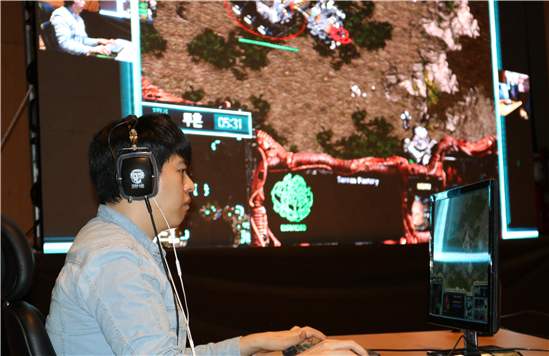
\includegraphics[width=0.5\textwidth]{fig/song_human_ai.png}
%  \caption{Professional player Byung-Gu Song playing against AI bots.}
%  \label{figureSong}
%\end{figure} 
